\chapter{Introduction}
\pagenumbering{arabic}  % 1, 2, 3, 4, ...
\setcounter{page}{1}

Electric energy has become one of the most important source of energy and is widely used resource in world, with ever increasing demand of the (any) resource it becomes more and more difficult to maintain the system and Power System is no exception. Power System has become a complex entity and has gone beyond the limit of manual operattion and control, which makes automation and "smart" control imparitive. This creates demand for new set of measurement, operation and control tools. Out of this tools measurement tools are the most fundamental building block of the modern power system, which is now also know as "smart grid". Measurement devices are "eyes" and "ears" in the system to the centralized "brain", operating-control-corrective system.  

In power system active power and frequency are the most important parameters to be monitored, flow of active power is decided by the phase angle of voltage between buses. Flow of active power decides the structure of network (transmission lines, capacity of devices etc) and hence accurate measurement of it has been of great interest since 1960-70s.\cite{agphadkebook}. Conventionally \textit{relative phase difference} between buses in the network was used, due to limitation of communication links, computational power and the economic pheasibility. This method(s) were slow, moderately accurate and dependent on a tones of heavy and/or manual calcualtion. 
After advancements in telecommunition technology and their speed \& reliability, better computation and satelite availability, trend of \textit{absolute phase difference} measurement came in to existance. The earliest system using absolute phase difference was reported in 1980 using LORAN-C satellite and HBG radio transmission for time reference. And during the same period Global Positioning System was being implemented by US DoD, which was immediately recognised as one of the best way of synchronising the power system, which brought the "Phasor Measurement" and "Synchrophasor" era in to existance. Lot of research was carried out and is being carried out in this area, and flurry of papers are available and are being published in different aspect of synchrophasor measurement. 
\section{Phasors, Synchrophasors and PMUs}
\subsection{Phasors: Defination}

In 1893 C. Steinmetz in his paper introduced simplified mathematcal description of a waveform of an alternating current electricity which he called as "phasor". In Physics and Engineering, \textit{phasor} is a complex number representing a sinusoidal quantity whose amplitude (A), angular velocity ($\omega$) and initial phase ($\phi$) are time-invarient.It is an analytic representation which decomposes sine function in to product of complex constants and a factor which encapsulates the frequency and time dependence. he complex constant, which encapsulates amplitude and phase dependence, is known as phasor, complex amplitude, and (in older texts) sinorx or even complexor.

Which Using Euler's formula can be represented mathematically as:
\begin{equation}\boldmath
Ae^{i(\omega t + \theta)} = A\cos(\omega t + \theta) + A\sin(\omega t + \theta)
\end{equation}

\subsection{Synchronised Phasors or Synchrophasors}
\begin{figure}
	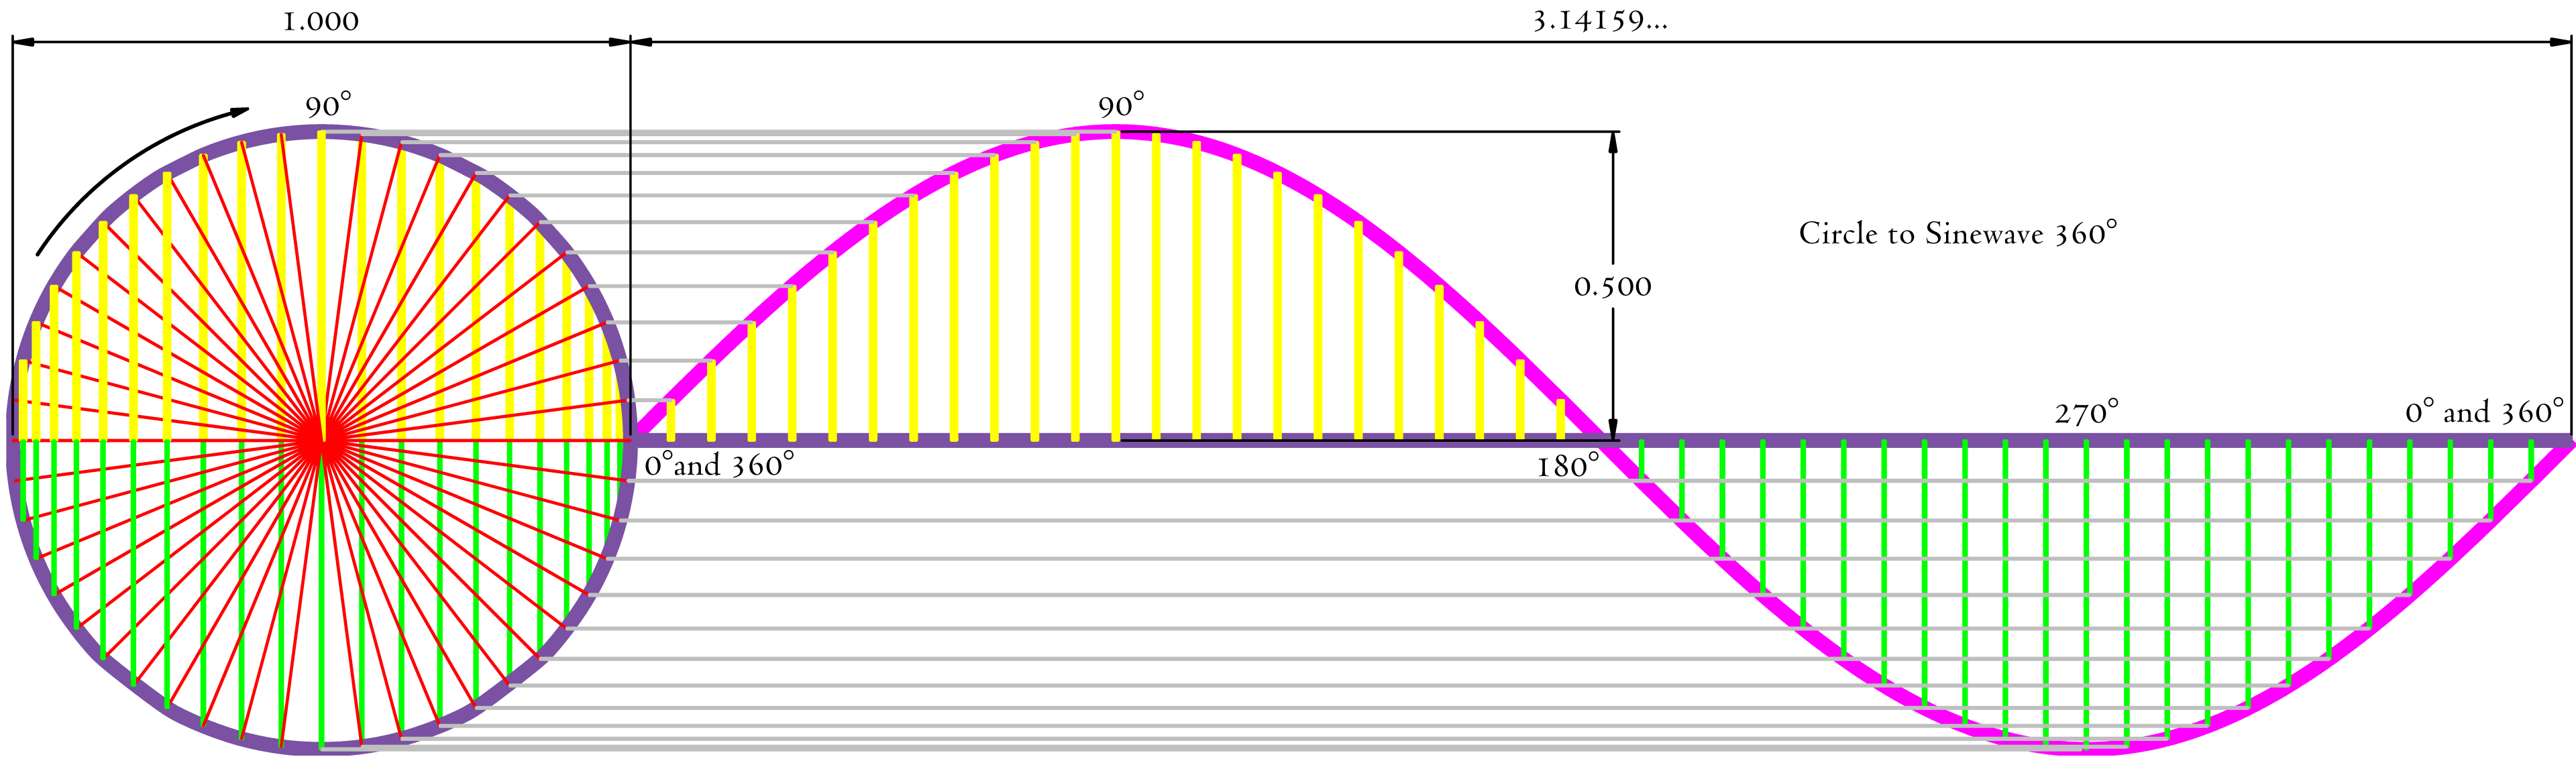
\includegraphics[width=\textwidth]{fig/Circle-To-Sine-Wave.png}
	\caption{Phasor Repsentation, Sampling and synchrophasor \cite{CirSinWave} .} 
	\label{fig:CirSin}
\end{figure}
 Synchronized sampling/measurement of sinusoidal complex quantity (phasor) at a precise reference (time) is called Synchronised Phasor. Time synchronization (of samples) allows synchronized real-time measurements of multiple remote location measurement points on the grid. And this resulting measurement is know as \textbf{synchrophasors} Fig. \ref{fig:CirSin}.
\subsection{Phasor Measurement Unit (PMU)}
PMU is a device which measures and estimates electrical wave in an power network using a common time source for sample synchronization. But it is important to note here that it is an ``estimate" of the phasor(!!) and not the actual measurement. 

This device was first invented by Dr. A. G. Phadke and Dr. James Thorp at Virginia Tech which is considered to be the first sucessful utilization of "phasors" for real-time phasors measurement that were synchronised with accurate absolute time reference provided by GPS.

\section{Wide Area Measurements}

Classically operation of grid was done by Supervisary Control And Data Acquizition(SCADA) system , which uses state estimator and other iterative solvers on system snapshot every 7-15 mins to measure and estimate the system operating point and phase angles. This approch is rather slow and less accurate but now after maturing of synchrophasor; Wide area monitoring systems (WAMS) have come in to existance, which are essentially based on the new data acquisition method of phasor estimation and allow monitoring of transmission system conditions over large areas and enable detecting and further counteracting grid instabilities. Importance and significance of synchrophasors and PMUs in WAMS can be understood when we see it from a practical perspective. Consider two geographically distant places like in India Kashmir and kaniyakumari or Aasam and Mumbai, How can we compute the phase difference of these two locations? if we want to scale the problem even further we can take American power grid where there exists Time Zone difference of 3 Hours (UTC-8.00 to UTC-5.00) from east coast to west coast, how can this be accomplished? This is where PMU and GPS comes into play, GPS enabled PMU provides an absolute time referenced \footnote{\url{http://www.physics.org/article-questions.asp?id=55}} voltage amplitude, angle and frequency (and maybe few other relevent) data of different bus to a regional control centre and eventually a central main control centre/system, this data samples are at a global reference (UTC, usually)\footnote{How accurate is GPS? know more: \url{http://www.gps.gov/systems/gps/performance/accuracy/}}. with an accuracy of few microseconds. All of this is available to the control centre at an rate of 12 to 25 snapshots per seconds, such high (and accurate) data (rate) enables system operator to operate the system efficiently and nearer to the operating limits and in case of contingencies enables them to take rapid corrective and/or preventive actions.
\begin{figure}
	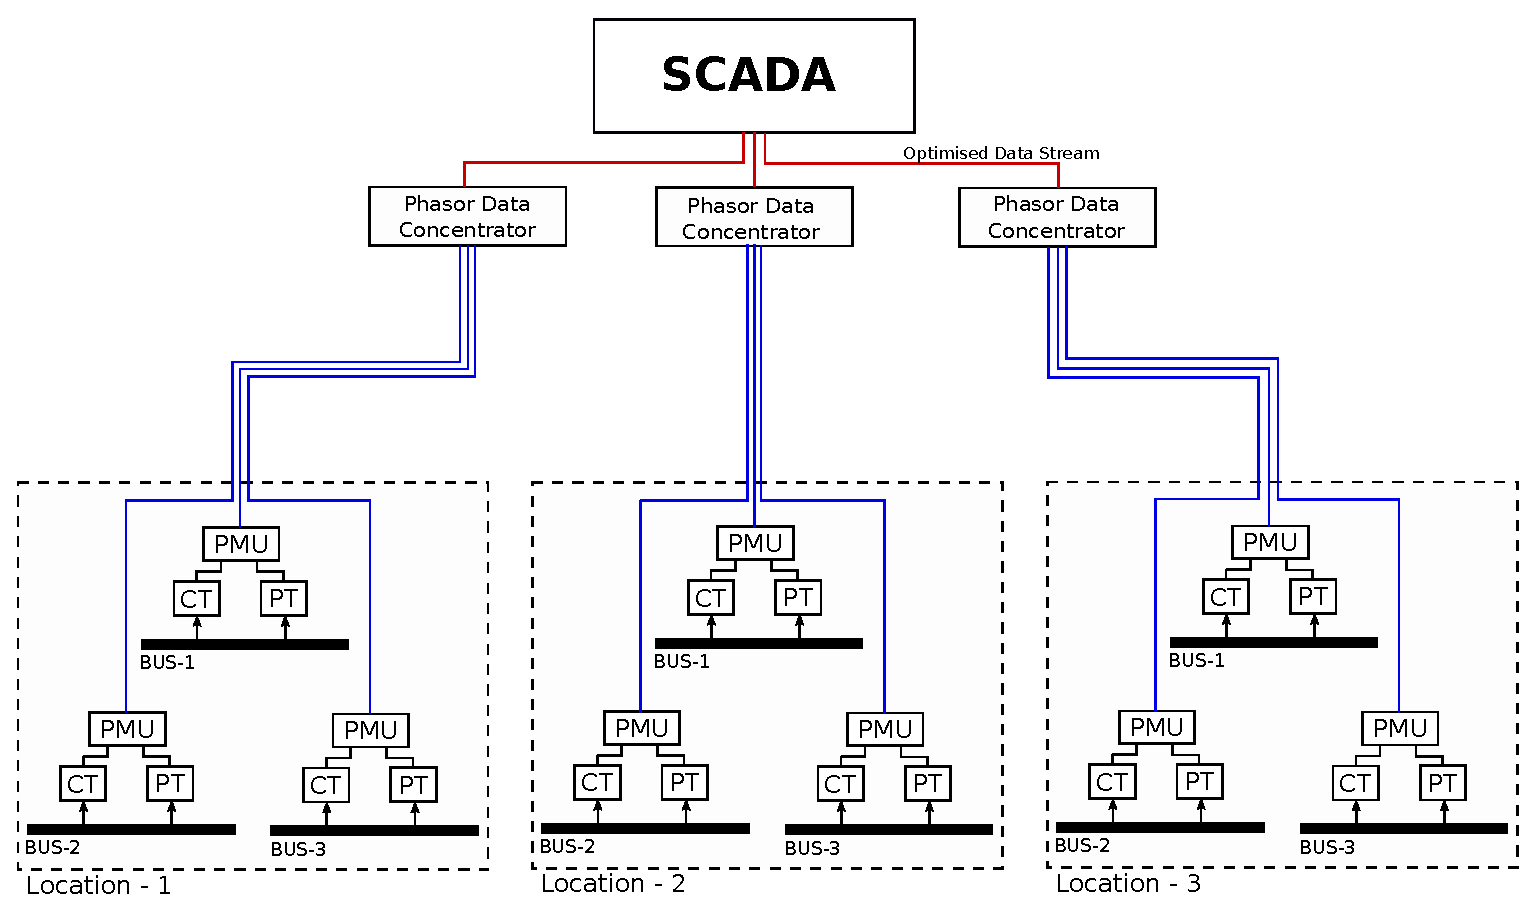
\includegraphics[width=\textwidth]{fig/wams.eps}
	\caption{Simplified structure of WAMS}
	\label{fig:wams}
\end{figure}

Fig. \ref{fig:wams} Shows a simplified architecture of modern Wide Area Measurement System. PMUs are installed at different substations on HV buses, via CTs and PTs, each PMU has multiple channels samplling AC waves at high rate. Rate of sampling varies according to the manufacturer and implementation of the scheme. Each PMU is provided a GPS receiver for accurate time with accuracy of approx 500 600 ns which is necessary for achiving time accuracy of 1-2 $\mu$s demanded by the standard. Each data after being samplled is then filtered using different DFT/FFT algorithm and is timestamped. This time stampped data is then sent to either SCADA or to a local Phasor Data Concentrator, which consolidates the data stream coming from different PMUs and send an bandwidth optimised data stream to the higher PDC or SCADA. 

